\subsection{Deep Learning Model Diagram}
\label{subsec:ml_diagram}
In this section, the process on how the deep learning model 
was developed is shown in Figure \ref{fig:ml_model}. 
Wherein, the process overview is based on the Fine-Tuned Support 
Vector Regression Model for Stock Predictions by 
\citeA{Dash2016}.
% Machine Learning Model Diagram
\begin{figure}[ht]
    \centering
    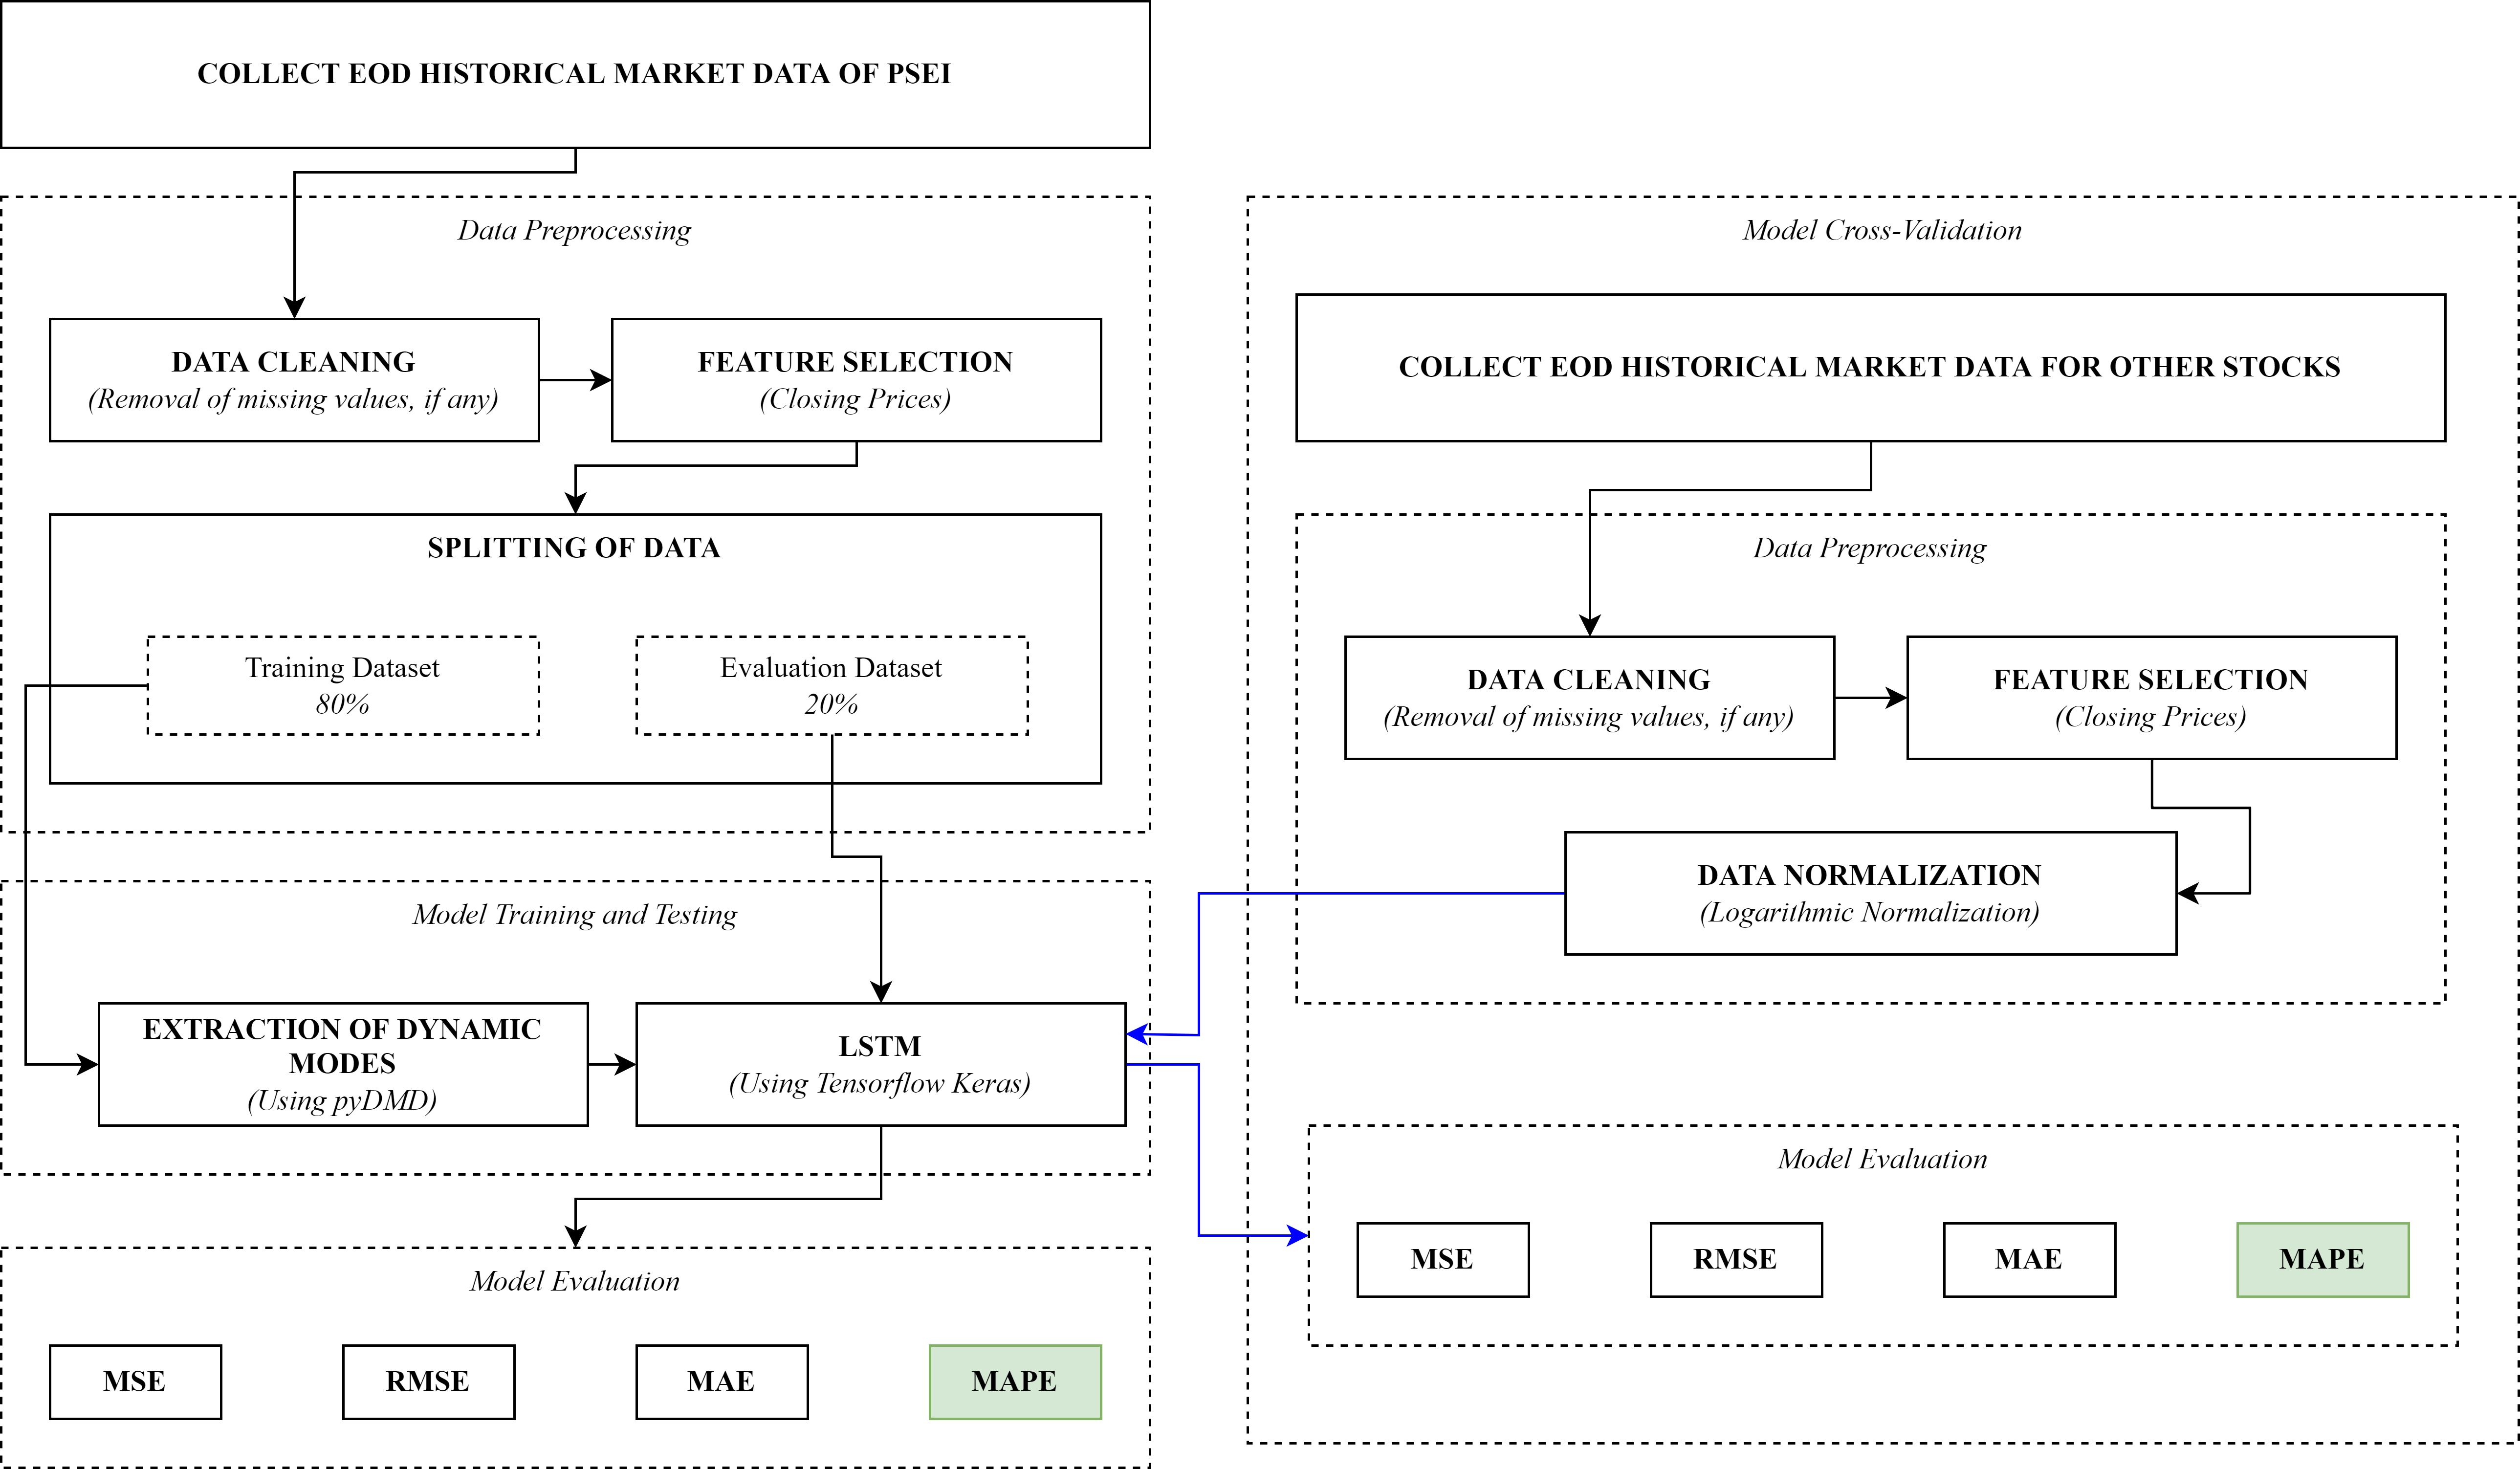
\includegraphics[width=1\textwidth]{./assets/Chapter_3/Machine Learning Model.png}
    \caption{DMD-LSTM Model Development Methodology for alamSYS}
    \label{fig:ml_model}
\end{figure}
\FloatBarrier

\subsubsection{Data Collection}
\label{subsubsec:model_data_collection}
The market data used to develop the DMD-LSTM model was obtained through EODHD's 
end-of-day market data API. While PSEI market data was used for model 
training and testing, market data from other stocks was used for cross-validation 
of the DMD-LSTM model. The following are the specifics of the stocks gathered:
\begin{longtable}{|c|c|c|c|}
    \caption{Collected Market Data Details}
    \label{tab:market_data_details}\\
    \hline
    \textbf{Stock} & \textbf{Data Count} & \textbf{Start Date} & \textbf{End Date} \\ \hline
    \endfirsthead
    %
    \multicolumn{4}{c}%
    {{\bfseries Table \thetable\ continued from previous page}} \\
    \hline
    \textbf{Stock} & \textbf{Data Count} & \textbf{Start Date} & \textbf{End Date} \\ \hline
    \endhead
    %
    \textbf{AC}    & 6809                & June 27, 1994       & February 10, 2023 \\ \hline
    \textbf{ALI}   & 6789                & June 27. 1994       & February 10, 2023 \\ \hline
    \textbf{AP}    & 3795                & July 16, 2007       & February 10, 2023 \\ \hline
    \textbf{BDO}   & 5041                & May 22, 2002        & February 10, 2023 \\ \hline
    \textbf{BLOOM} & 3033                & October 30, 2000    & February 10, 2023 \\ \hline
    \textbf{FGEN}  & 4142                & February 02, 2006   & February 10, 2023 \\ \hline
    \textbf{GLO}   & 6707                & January 03, 1995    & February 10, 2023 \\ \hline
    \textbf{ICT}   & 6805                & January 03, 1995    & February 10, 2023 \\ \hline
    \textbf{JGS}   & 6525                & June 27, 1994       & February 10, 2023 \\ \hline
    \textbf{LTG}   & 3774                & February 06, 1995   & February 10, 2023 \\ \hline
    \textbf{MEG}   & 6751                & January 03, 1995    & February 10, 2023 \\ \hline
    \textbf{MER}   & 6799                & June 27, 1994       & February 10, 2023 \\ \hline
    \textbf{MPI}   & 3888                & December 18, 2006   & February 10, 2023 \\ \hline
    \textbf{PGOLD} & 2762                & October 06, 2011    & February 10, 2023 \\ \hline
    \rowcolor[HTML]{9AFF99} 
    \textbf{PSEI}  & 5675                & January 03, 2000    & February 10, 2023 \\ \hline
    \textbf{RLC}   & 5879                & June 27, 1994       & February 10, 2023 \\ \hline
    \textbf{RRHI}  & 2253                & November 11, 2013   & February 10, 2023 \\ \hline
    \textbf{SMC}   & 6799                & June 27. 1994       & February 10, 2023 \\ \hline
    \textbf{TEL}   & 6814                & June 27, 1994       & February 10, 2023 \\ \hline
    \textbf{URC}   & 6135                & June 03, 1995       & February 10, 2023 \\ \hline
\end{longtable}

\subsubsection{Data Preprocessing}
\label{subsubsec:model_data_processing}
Data preprocessing before model training and testing is composed of three main processes which are as follows:
\begin{itemize}
    \item[(a)] Data Cleaning - This was done to clean any missing values from the data.
    \item[(b)] Feature Selection - Closing prices was selected as the main feature of the model.
    \item[(c)] Splitting of Data - Data was split in the ratio of 80:20 for testing and training data, respectively.
\end{itemize}
\hfill \\
Meanwhile for the data preprocessing for cross-validation, the following processes were done:
\begin{itemize}
    \item[(a)] Data Cleaning - This was done to clean any missing values from the data.
    \item[(b)] Feature Selection - Closing prices was selected as the main feature of the model.
    \item[(c)] Data Normalization - Using logarithmic normalization method, the data was normalized.
    Logarithmic normalization was utilized to help solved the problem with the data having extreme ranges,
    which affects the evaluation of the cross-validation. In essence it was used to enable data stability, and
    increase interpretability \cite{Baeldung2022, Bex2021, Andrew2019}.
\end{itemize}

\subsubsection{Model Training and Testing}
\label{subsubsec:model_training_testing}
Using pyDMD the dynamic modes was extracted from the training and testing data,
these extracted values alongside the actual closing price data were utilized for
the training of an LSTM model using Tensorflow Keras Library.
\hfill \\

There are a total of eight model variations trained and tested, which are as follows:
(1) Baseline LSTM with window size of 5;
(2) Baseline LSTM with window size of 10;
(3) Baseline LSTM with window size of 15;
(4) Baseline LSTM with window size of 20;
(5) DMD-LSTM with window size of 5;
(6) DMD-LSTM with window size of 10;
(7) DMD-LSTM with window size of 15; and
(8) DMD-LSTM with window size of 20.
Where the best performing model was used for the cross-validation and was deployed to the system.


\subsubsection{Model Evaluation}
\label{subsubsec:model_evaluation}
The DMD-LSTM Model was evaluated using the following error metrics:
\begin{itemize}
    \item[(a)] Mean Squared Error (MSE) - MSE is a well-known metric for assessing regression models. 
    It calculates the average of the squared differences between predicted and true values. 
    MSE is useful because it penalizes large errors more severely than small errors, 
    which is important in some applications. A lower MSE indicates that the model performed better
    \cite{StephMSE}.
    \item[(b)] Root Mean Squared Error (RMSE) - Another popular metric for evaluating regression models 
    is the RMSE, which is the square root of the MSE. It, like MSE, computes the average of the 
    differences between predicted and true values. Because it is in the same unit as the target variable, 
    RMSE is easier to interpret. A lower RMSE indicates that the model is performing better
    \cite{StephRMSE}.
    \item[(c)] Mean Absolute Error (MAE) - It calculates the average of the absolute differences 
    between predicted and true values. MAE is advantageous because it is more resistant to 
    outliers than MSE and RMSE. A lower MAE indicates that the model is performing better
    \cite{SecretDataScientistMAE}.
    \item[(d)] Mean Absolute Percentage Error (MAPE) - It computes the average percentage difference 
    between predicted and true values. MAPE is useful because it provides a relative measure of error, 
    which makes comparing model performance across different target variable scales easier. 
    A lower MAPE indicates that the model is performing better
    \cite{Allwright2022MAPE}.
    Furthermore, this is the primary error metric used to select the final model deployed to alamSYS.
\end{itemize}

\subsubsection{Model Cross-Validation}
\label{subsubsec:model_cross_validation}
The model selected for the cross-validation was the DMD-LSTM model with a window size of 5, due to it
being the highest performing model based on having the lowest MAPE scores compared to the other models,
this is further discussed on Chapter 4 of this paper.
\hfill \\

The cross-validation was conducted using the stock market data from the other stocks aside from the
training data from PSEI. Where cross-validation of an LSTM model must be done before deployment 
to assess the model's generalization performance. LSTM models are well-known for their ability 
to capture long-term dependencies in sequential data, but their performance varies greatly depending 
on the dataset and model hyperparameters used. And a correctly performed cross-validation helps to 
provide a more accurate estimate of the model's performance on unseen data, which is critical 
for ensuring that the model performs well in real-world scenarios
\cite{Mellema2020, DBLP:journals/corr/abs-1908-06272}.

\subsubsection{Model Deployment}
\label{subsubsec:model_deployment}
After determining that the DMD-LSTM model works well with non-training stock market data, 
it was deployed to the alamSYS as a '.keras' file.